\documentclass[a4paper]{report}

%====================== PACKAGES ======================

\usepackage[french]{babel}
\usepackage[utf8x]{inputenc}
%pour gérer les positionnement d'images
\usepackage{float}
\usepackage{amsmath}
\usepackage{graphicx}
\usepackage[colorinlistoftodos]{todonotes}
\usepackage{url}
%pour les informations sur un document compilé en PDF et les liens externes / internes
\usepackage{hyperref}
%pour la mise en page des tableaux
\usepackage{array}
\usepackage{tabularx}
%pour utiliser \floatbarrier
%\usepackage{placeins}
%\usepackage{floatrow}
%espacement entre les lignes
\usepackage{setspace}
%modifier la mise en page de l'abstract
\usepackage{abstract}
%police et mise en page (marges) du document
\usepackage[T1]{fontenc}
\usepackage[top=2cm, bottom=2cm, left=2cm, right=2cm]{geometry}
%Pour les galerie d'images
\usepackage{subfig}

%====================== INFORMATION ET REGLES ======================

%rajouter les numérotation pour les \paragraphe et \subparagraphe
\setcounter{secnumdepth}{4}
\setcounter{tocdepth}{4}

\hypersetup{							% Information sur le document
pdfauthor = {Enzo Durand,
			Thomas Gignoux},			% Auteurs
pdftitle = {Jeu d’infection -
			Sécurité et aide à la décision}
			}

%======================== DEBUT DU DOCUMENT ========================

\begin{document}

%régler l'espacement entre les lignes
\newcommand{\HRule}{\rule{\linewidth}{0.5mm}}

%page de garde
\begin{titlepage}
\begin{center}


\includegraphics[width=0.35\textwidth]{./logo}~\\[1cm]

\textsc{\LARGE Université de Caen Normandie}\\[1.5cm]

\textsc{\Large L2 Informatique }\\[1.5cm]

\HRule \\[0.4cm]

{\huge \bfseries Sécurité et aide à la décision \\
 Jeu d’infection \\[0.4cm] }

\HRule \\[1.5cm]

\begin{minipage}{0.4\textwidth}
\begin{flushleft} \large
\emph{Membre du groupe:}\\
Enzo Durand\\
Thomas Gignoux\\


\end{flushleft}
\end{minipage}
\begin{minipage}{0.4\textwidth}
\begin{flushright} \large
\emph{Enseignant:} \\
Grégory \textsc{Bonnet}\\
\end{flushright}
\end{minipage}

\vfill

{\large \today}

\end{center}
\end{titlepage}
\tableofcontents
\thispagestyle{empty}
\setcounter{page}{0}
%ne pas numéroter le sommaire


%espacement entre les lignes d'un tableau
\renewcommand{\arraystretch}{1.5}

%====================== INCLUSION DES PARTIES ======================

~
\thispagestyle{empty}
%recommencer la numérotation des pages à "1"
\setcounter{page}{0}
\newpage

\chapter{Introduction}

\section{Présentation du projet}
\flushleft Nous avons programmé un jeu dont les règles étaient données : 

"Soit une grille de N × M cases. Chaque joueur Blanc et Noir débute la partie avec un
pion, respectivement en bas à droite et en haut à gauche. L'objectif du jeu est de posséder en
fin de partie le plus de pion possible, la partie se terminant lorsque l'un des joueurs ne dispose
plus de pion, ou si aucun joueur ne peut faire de coups légaux. À chaque tour, le joueur actif
choisit un pion et effectue une des actions suivantes avant de passer la main à son adversaire :\\
— Dupliquer le pion en en plaçant un nouveau sur une case libre à une distance de un dans
une des quatre directions cardinales (haut, bas, gauche ou droite). Tout pion adverse 
en contact avec ce nouveau pion est transformé en pion du joueur. \\
— Déplacer le pion sur une case libre à une distance de deux dans une des quatre directions
cardinale ; ce mouvement permet de sauter par-dessous un autre pion (quel qu'en soit
le propriétaire)."
\\[0.5 cm]
Le but étant, une fois avoir programmé ce jeu, d'implémenter un algorithme appelé "MinMax" ainsi
qu'un algorithme permettant d'optimiser MinMax en explorant moins de possibilités. Après avoir implémenté
ces deux algorithmes à notre jeu, nous avons analysé les données par partie ou sur plusieurs parties.
Nous avons fait une interface graphique permettant d'afficher différentes courbes extraites d'une partie.
Nous avons aussi créer un tableur et récupéré des données sur plusieurs parties. \\


Voici les différentes classes de notre programme: \\
\begin{figure}[!ht]
\begin{center}
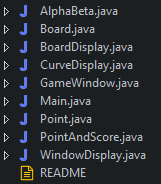
\includegraphics[width=0.40\textwidth]{./ARBORESCENCE}~\\
\end{center}
\end{figure}
\newpage


Ainsi que les différentes méthodes de notre class Board
\begin{figure}[!ht]
\begin{center}
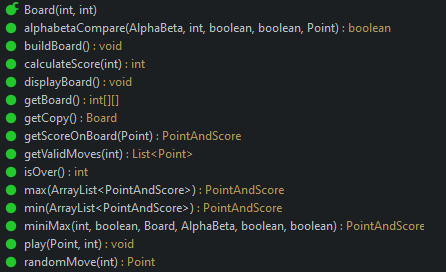
\includegraphics[width=0.65\textwidth]{./METHODESBOARD}
\end{center}
\end{figure}
\\
Et voici comment se présente le déroulement de la partie dans la console.
\begin{figure}[!ht]
\begin{center}
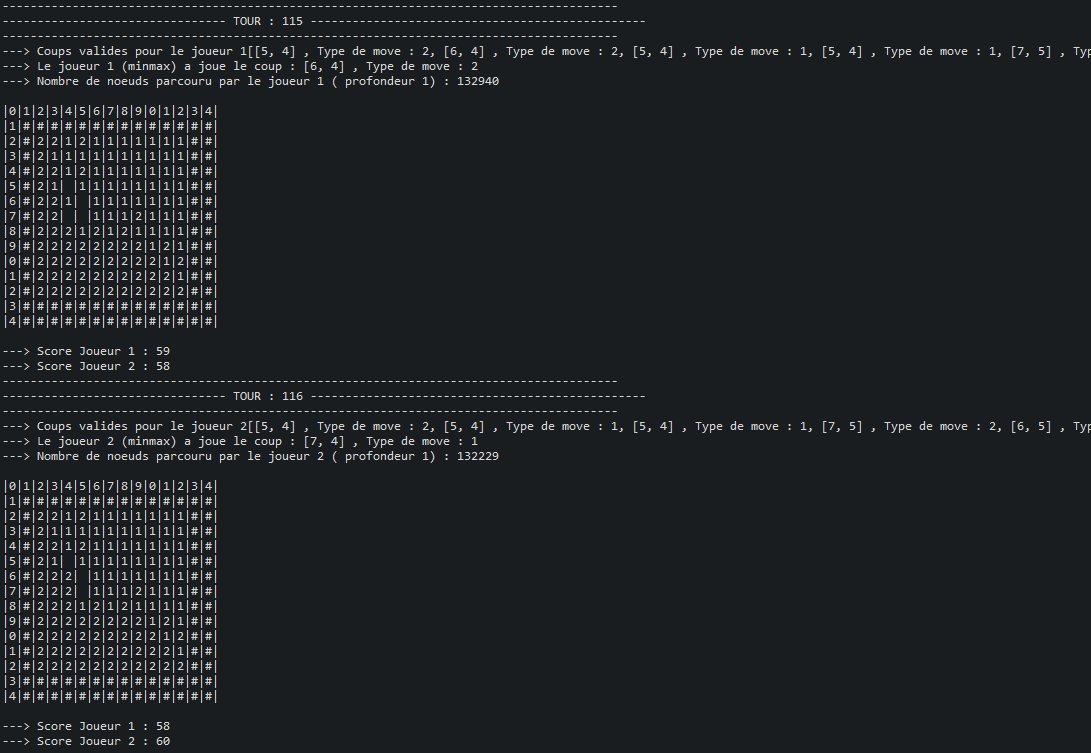
\includegraphics[width=0.95\textwidth]{./INTROJEU}
\end{center}
\end{figure}





\chapter{Algorithme}


\section{Minimax}

\flushleft Dans une première partie nous nous sommes
intéressés au minmax de profondeur 0, cet algorithme permettait de jouer mais sans récursivité, il
ne fonctionnait donc pas en profondeur 1 et plus. Après avoir réussit à faire cet algorithme, nous
avons travaillé sur l'implémentation de la récursivité de cet algorithme.


Au début nous nous étions précipités sur le jeu, l'implémentation de MinMax était donc incompatible
avec notre jeu. Nous avons donc tout supprimé pour recommencer sur de meilleur base.
Après avoir reprogrammé le jeu de base, l'implémentation de MinMax était plus facile.

Les captures d'écrans suivantes sont des tentatives avant d'arriver au minmax final.
\begin{figure}[!ht]
\begin{center}
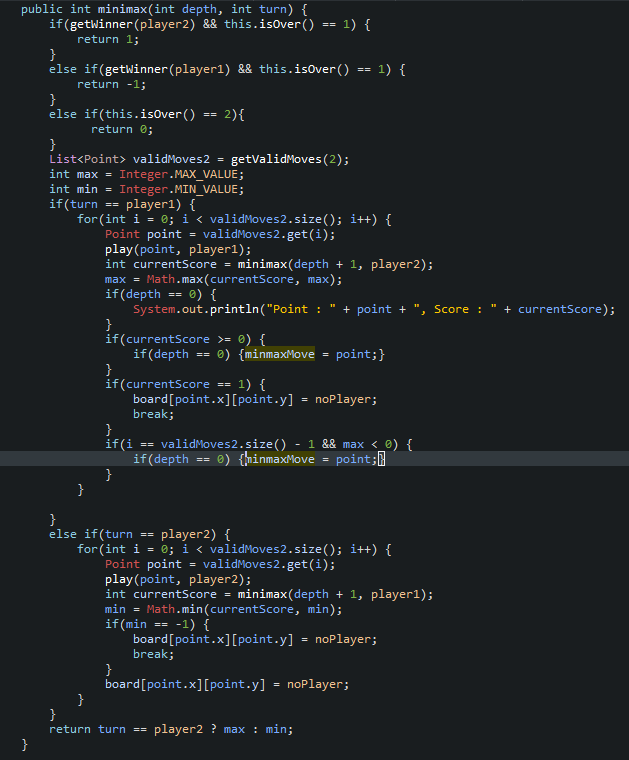
\includegraphics[width=0.65\textwidth]{./MINMAXDEBUT1}
\end{center}
\end{figure}
\newpage

\begin{figure}[!ht]
\begin{center}
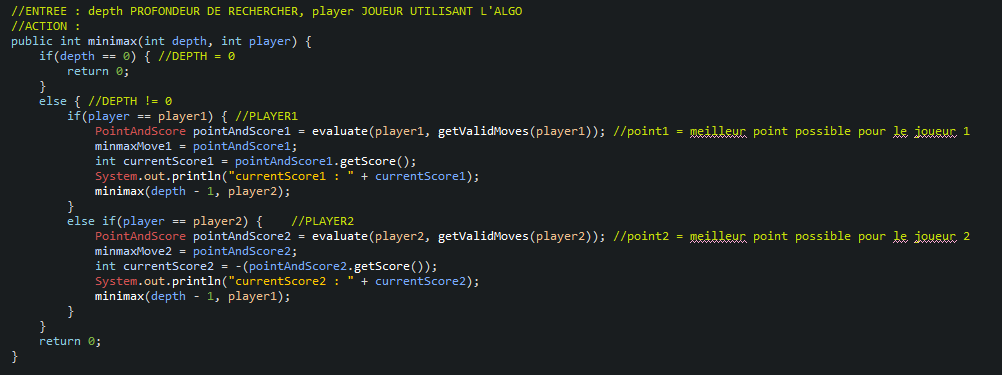
\includegraphics[width=0.85\textwidth]{./MINMAXDEBUT2}
\end{center}
\end{figure}

\centering \textbf{Après avoir vraiment compris l'algorithme en général, et après plusieurs tentatives nous avons
réussit a implémenter l'algorithme et à le debugger.} \\ 


\centering \textbf{La capture d'écran suivante est notre MinMax final.}

\begin{figure}[!ht]
\begin{center}
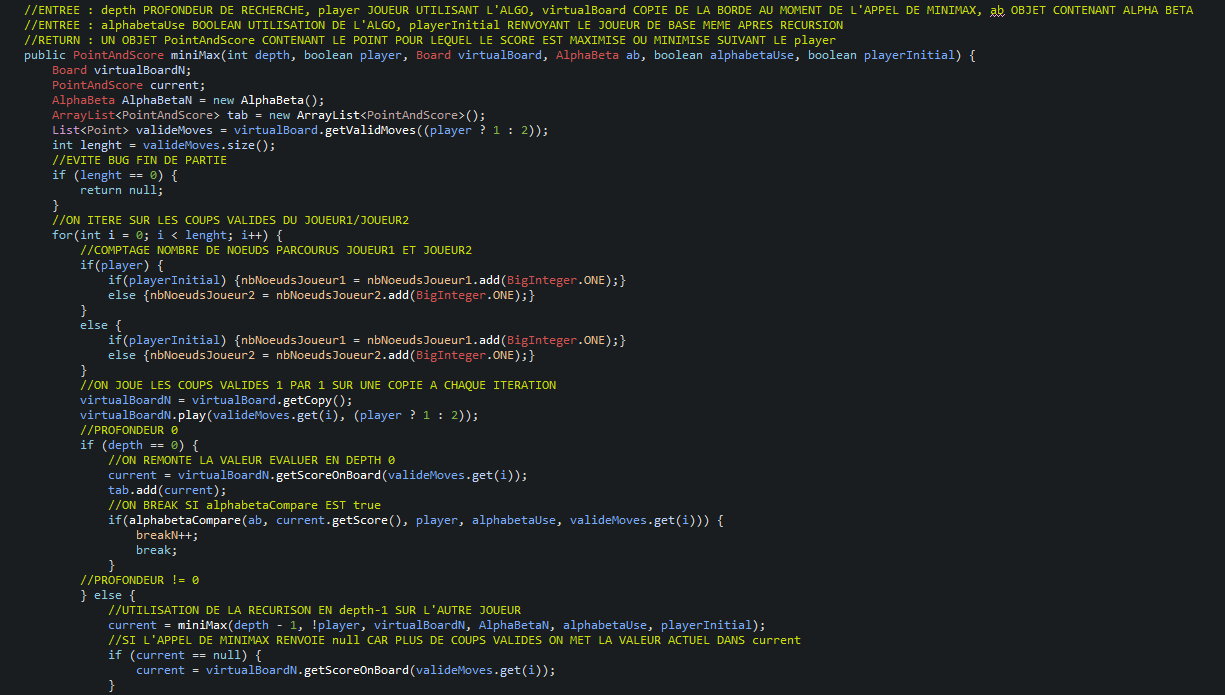
\includegraphics[width=0.95\textwidth]{./MINMAX1} 
\end{center}
\end{figure}

\begin{figure}[!ht]
\begin{center}
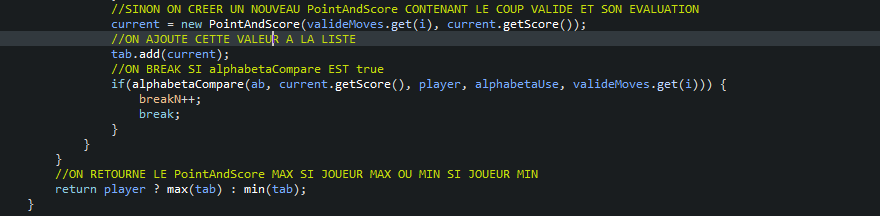
\includegraphics[width=0.75\textwidth]{./MINMAX2}
\end{center}
\end{figure}

\begin{figure}[!ht]
\begin{center}
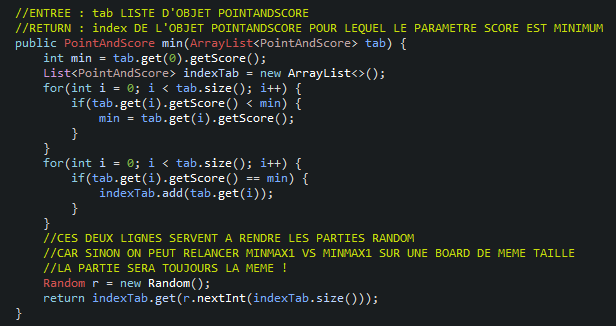
\includegraphics[width=0.65\textwidth]{./MIN}
\end{center}
\end{figure}

\begin{figure}[!ht]
\begin{center}
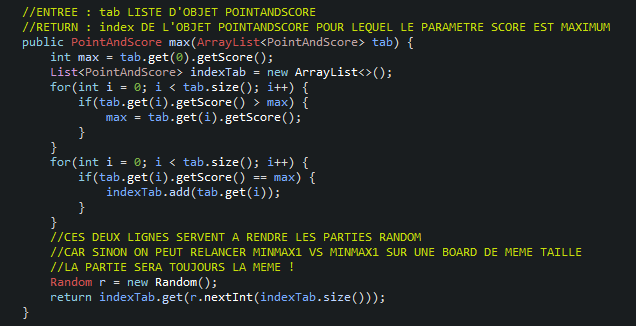
\includegraphics[width=0.65\textwidth]{./MAX}
\end{center}
\end{figure}

\newpage

\section{AlphaBeta}

L'algorithme AlphaBeta semblait plutôt simple après avoir implémenter MinMax.
Nous avons donc essayé de l'implémenter puis de le debugger mais le nombre d'informations
même sur une petite grille et une petite profondeur de minmax rendait le problème complexe.
Après plusieurs tentatives nous n'avons pas réussit à implémenter AlphaBeta.
Le problème étant peu être la structure de MinMax, il y a surement besoin de changer MinMax
afin de pouvoir implémenter AlphaBeta. Le problème semble être lié la récursivité.

\begin{figure}[!ht]
\begin{center}
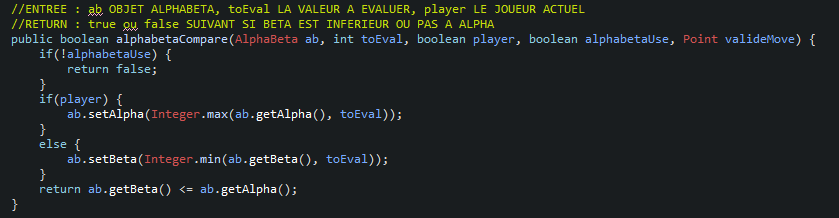
\includegraphics[width=0.90\textwidth]{./ALPHABETA}
\end{center}
\end{figure}



\chapter{Analyse de données }

\section{Nombre de nœuds}
\subsection{Par tour}
\flushleft Pour pouvoir analyser le nombre de nœuds explorés pendant une partie par un joueur utilisant MinMax,
nous avons implémenter une interface graphique qui trace une courbe à la fin de la partie.
Nous avons donc lancé plusieurs parties puis nous avons tracé les courbes suivant le nombre de tour.
Les courbes suivantes sont des courbes représentant le nombre total de nœuds parcourus par tour ainsi 
que les courbes représentant le nombre de nœuds à chaque tours.

On voit sur les premières types de courbes que au début de la partie il n'y a pas beaucoup de nœuds
parcourus car il y a peu de pions sur la grille donc peu de possibilités. Ensuite le nombre de nœuds
accélère rapidement car il y a de plus en plus de possibilités. A la fin de la partie le nombre de nœuds
redescend car il n'y a plus beaucoup de place libres dans la grille donc peu de coups valides.


\begin{figure}[!ht]
\begin{center}
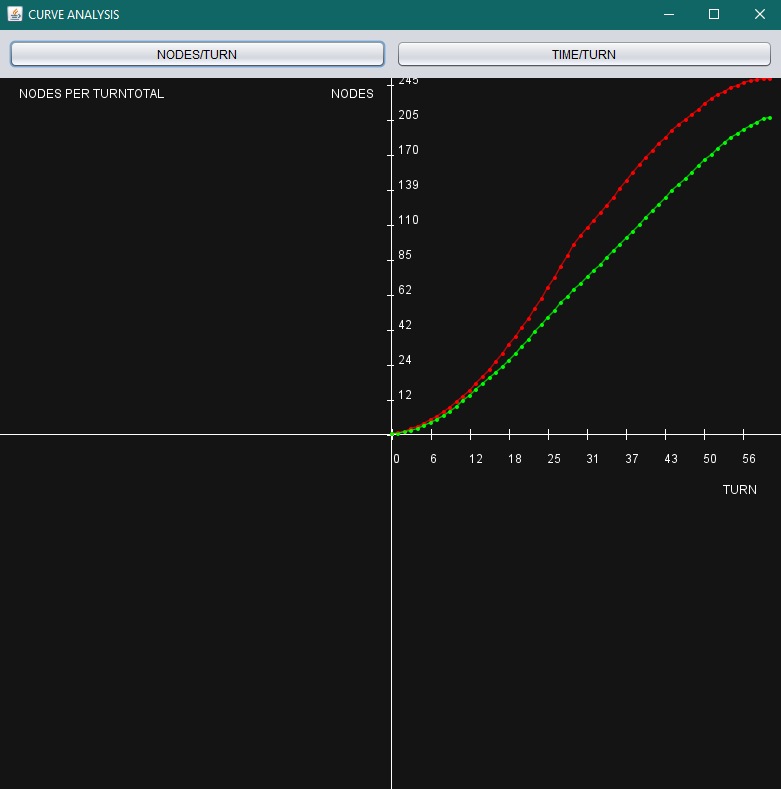
\includegraphics[width=0.60\textwidth]{./NODESPERTURN0}
\end{center}
\end{figure}
\newpage

\begin{figure}[!ht]
\begin{center}
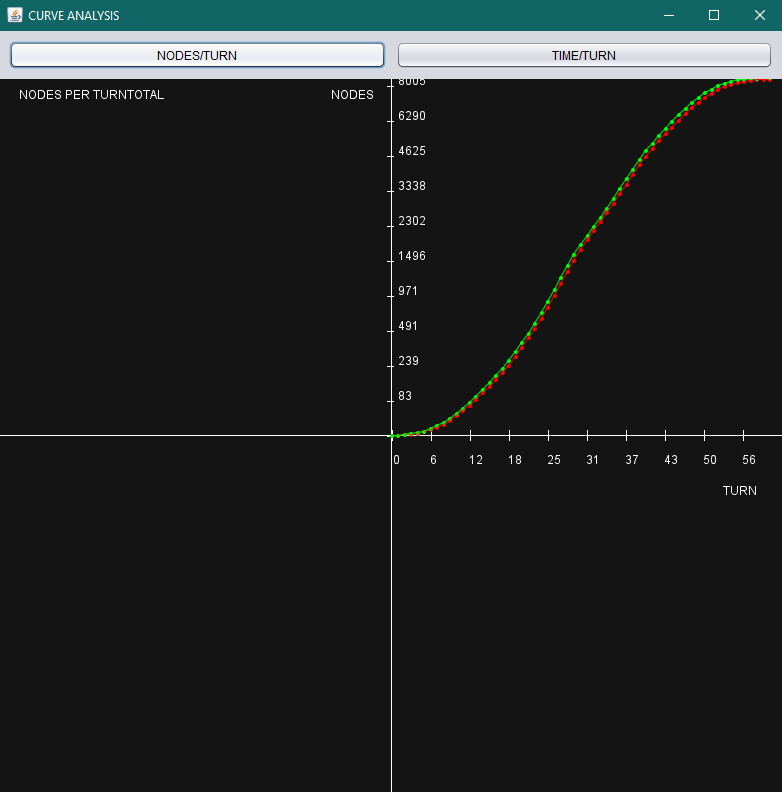
\includegraphics[width=0.60\textwidth]{./NODESPERTURN1}
\end{center}
\end{figure}

\begin{figure}[!ht]
\begin{center}
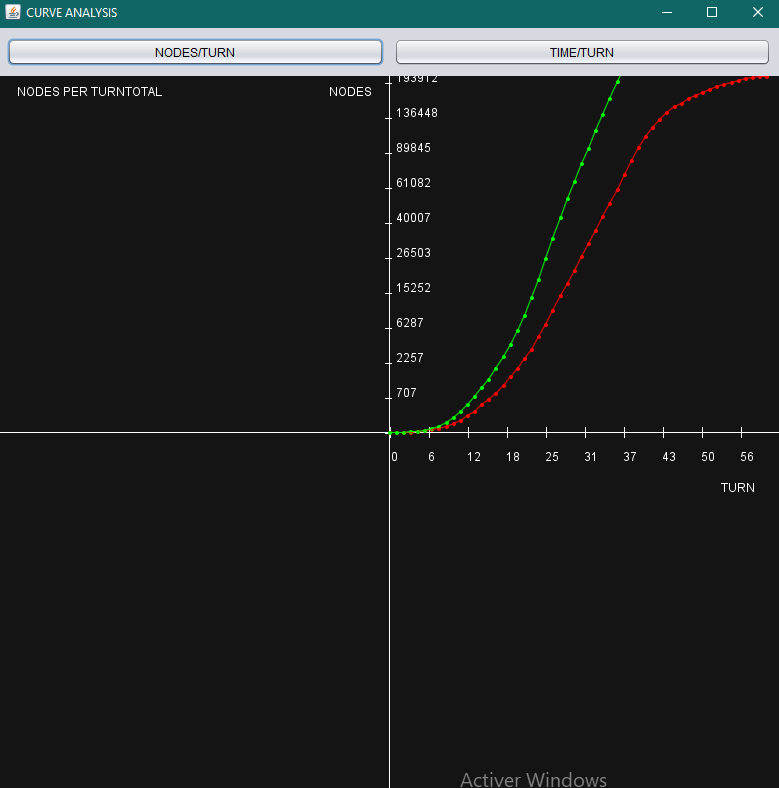
\includegraphics[width=0.60\textwidth]{./NODESPERTURN2}
\end{center}
\end{figure}
\newpage

\begin{figure}[!ht]
\begin{center}
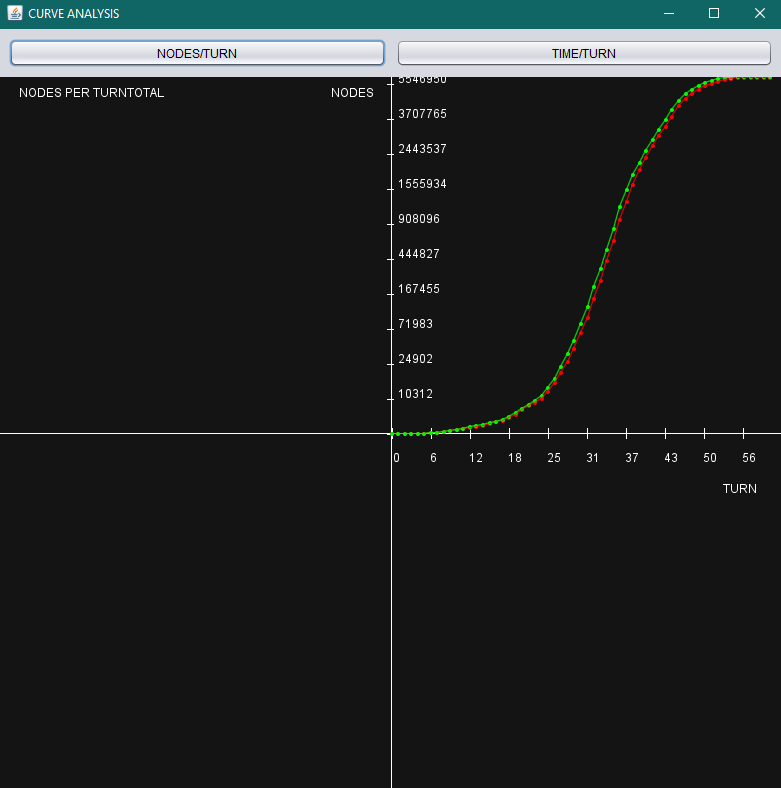
\includegraphics[width=0.60\textwidth]{./NODESPERTURN3}
\end{center}
\end{figure}

\begin{figure}[!ht]
\begin{center}
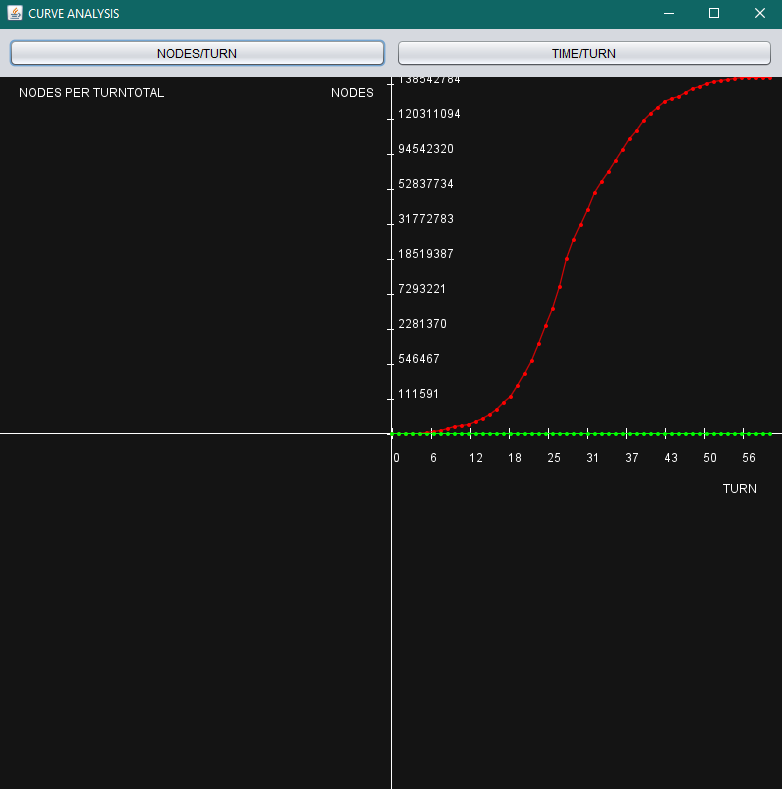
\includegraphics[width=0.60\textwidth]{./NODESPERTURN4}
\end{center}
\end{figure}
\newpage

\textbf{Sur les deuxièmes types de courbes nous voyons le même processus mais sous un autre angle.}

\begin{figure}[!ht]
\begin{center}
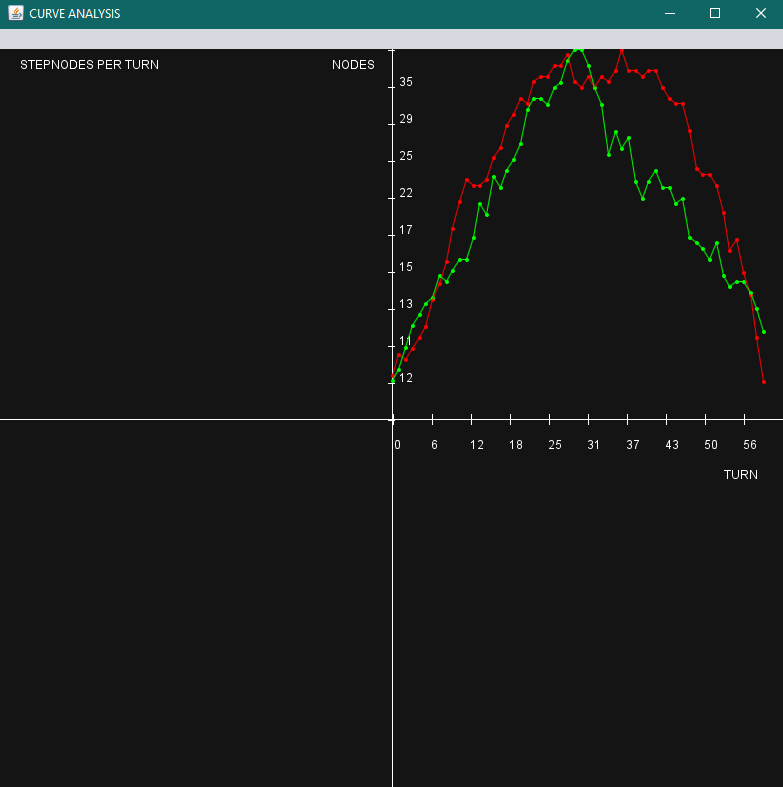
\includegraphics[width=0.60\textwidth]{./STEPNODESPERTURN0}
\end{center}
\end{figure}

\begin{figure}[!ht]
\begin{center}
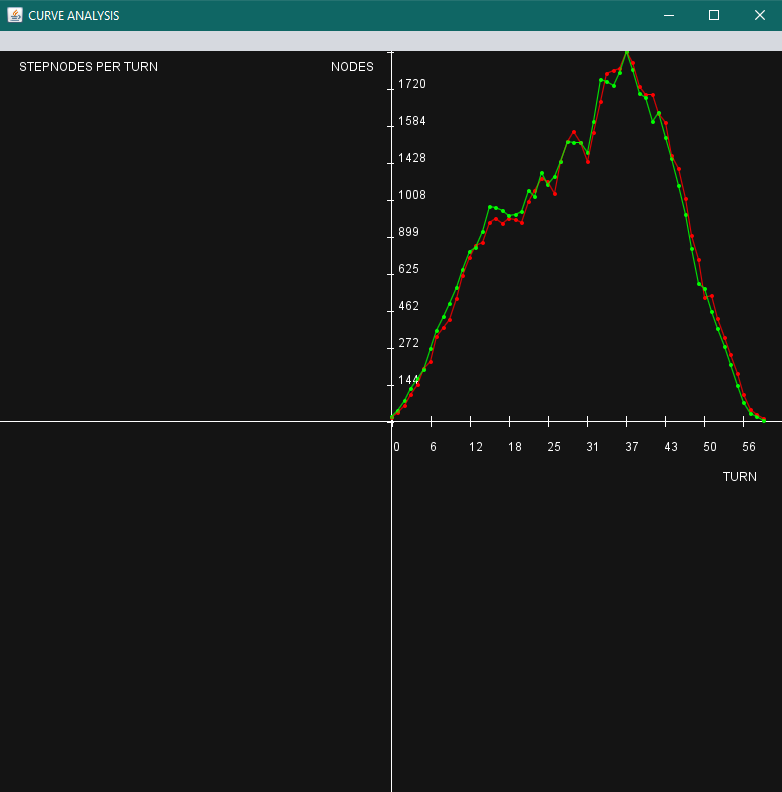
\includegraphics[width=0.60\textwidth]{./STEPNODESPERTURN1}
\end{center}
\end{figure}
\newpage

\begin{figure}[!ht]
\begin{center}
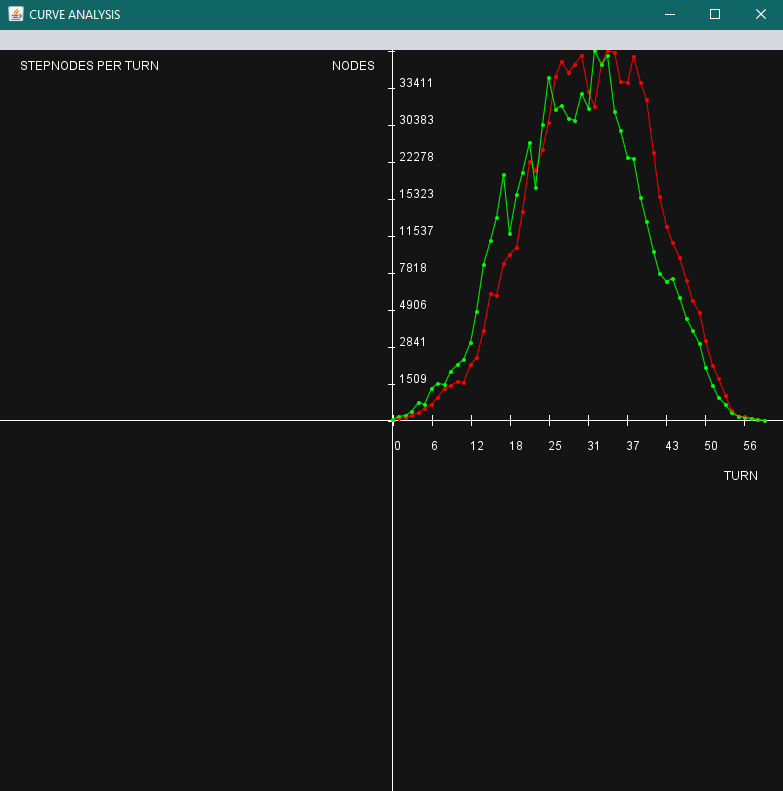
\includegraphics[width=0.60\textwidth]{./STEPNODESPERTURN2}
\end{center}
\end{figure}

\begin{figure}[!ht]
\begin{center}
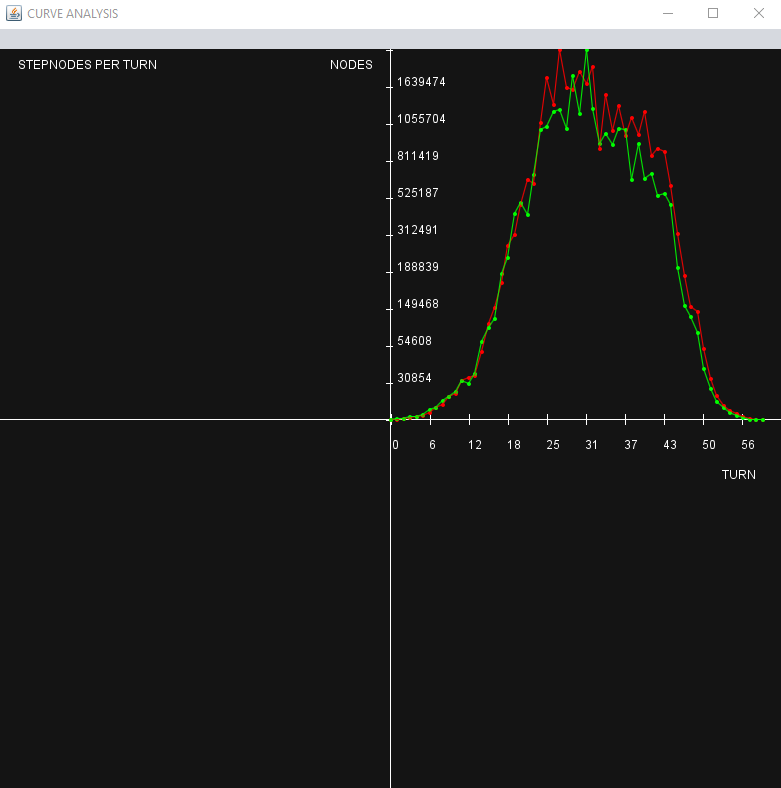
\includegraphics[width=0.60\textwidth]{./STEPNODESPERTURN3}
\end{center}
\end{figure}

\newpage

\begin{figure}[!ht]
\begin{center}
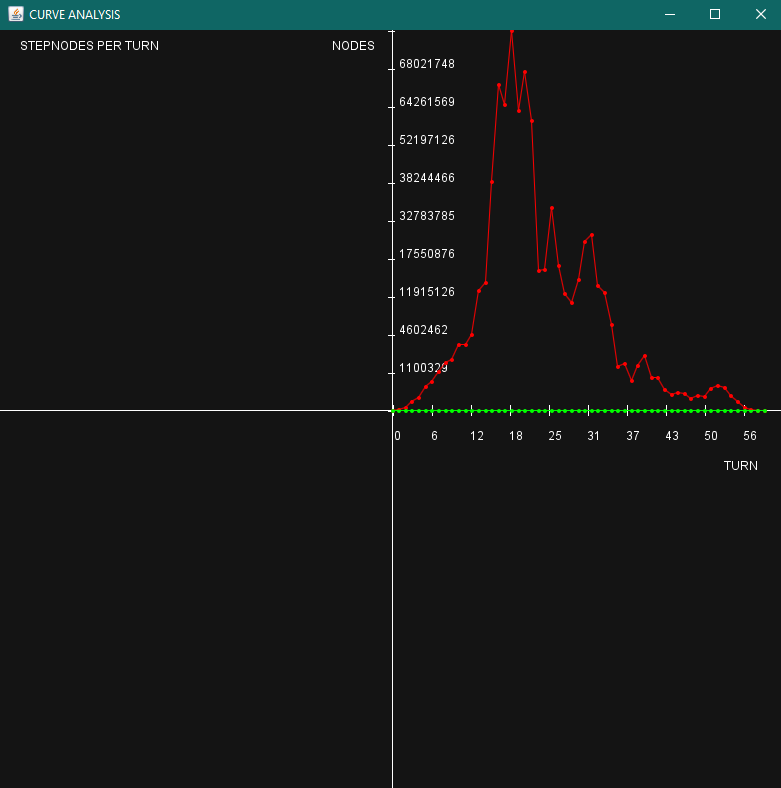
\includegraphics[width=0.65\textwidth]{./STEPNODESPERTURN4}
\end{center}
\end{figure}

Si nous avions réussit à implémenter alphabeta nous aurions tracé les courbes avec deux joueurs de même
profondeur minmax, mais l'un avec alphabeta activé et l'autre sans.
Nous aurions donc observé que la courbe du joueur avec alphabeta activé aurait été en dessous de l'autre
joueur.

\newpage

\subsection{Par profondeur}

Pour comprendre à quel point le nombre de nœuds croît suivant la profondeur donnée à l'algorithme,
nous avons tracé les courbes des nombres de nœuds totaux par rapport à la profondeur donnée à
MinMax. \\[0.75 cm]

 
\centering \textbf{Profondeur 0}
\begin{figure}[!ht]
\begin{center}
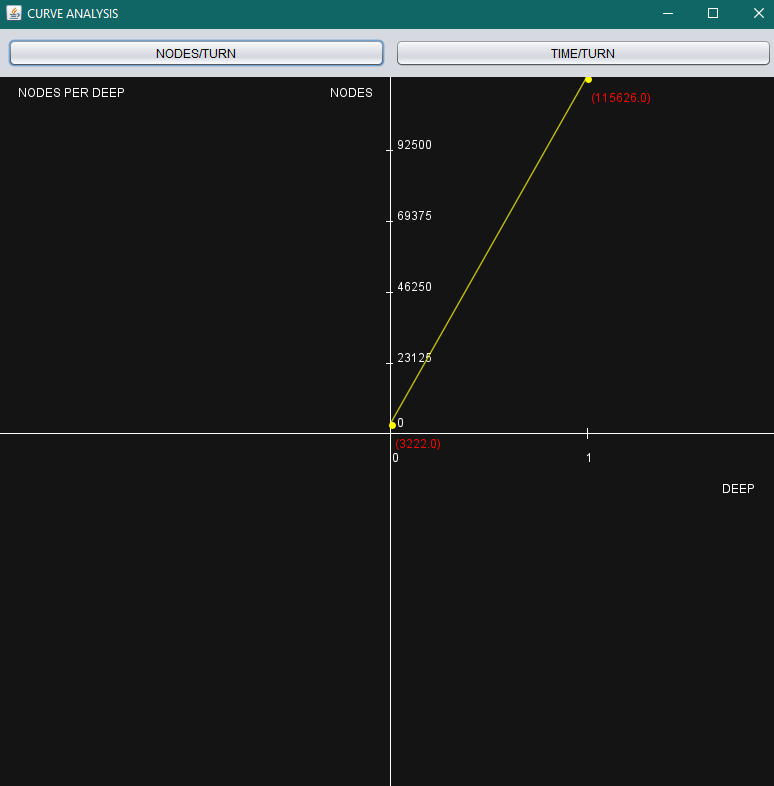
\includegraphics[width=0.60\textwidth]{./NODESPERDEEP1}
\end{center}
\end{figure}

\centering \textbf{Profondeur 1}
\begin{figure}[!ht]
\begin{center}
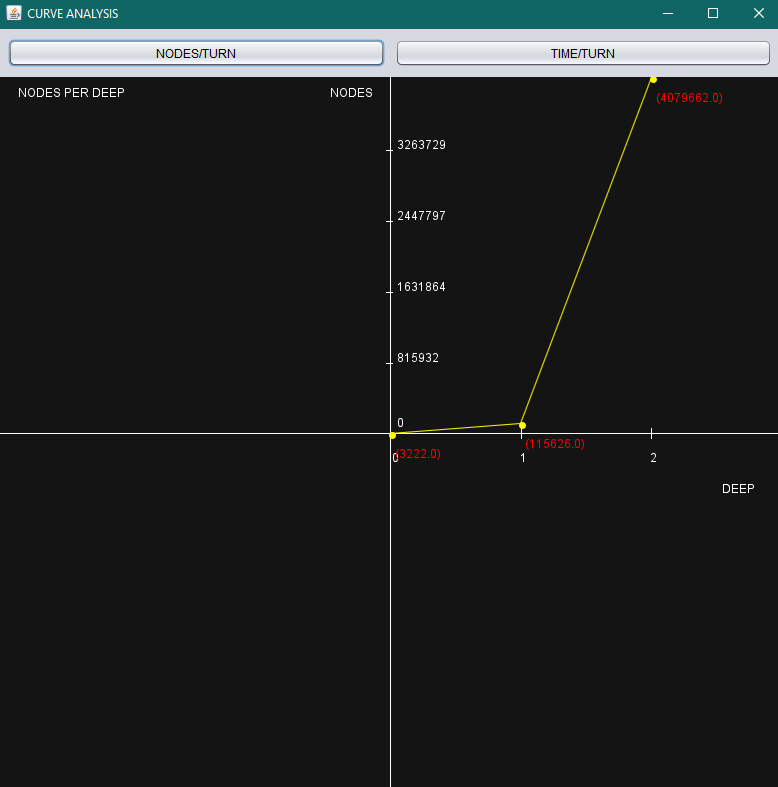
\includegraphics[width=0.60\textwidth]{./NODESPERDEEP2}
\end{center}
\end{figure}
\newpage

\centering \textbf{Profondeur 3}
\begin{figure}[!ht]
\begin{center}
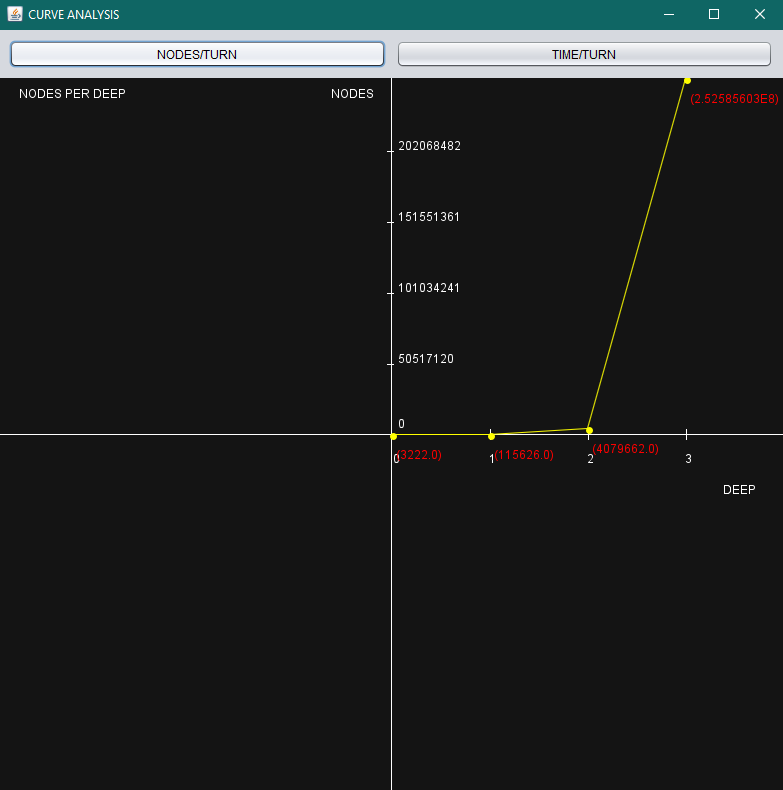
\includegraphics[width=0.60\textwidth]{./NODESPERDEEP3}
\end{center}
\end{figure}

Nous observons ici des courbes exponentiels, ceci étant logique vu que le nombre de nœuds explorés
est égale à: CoupsValidesAvecTour\up{profondeur} 
\newpage


\section{Taux de victoire par rapport a la profondeur et au nombre de coups d'avance}
Les captures suivantes sont des analyses de plusieurs parties suivant la profondeur et le nombre
de coups d'avance.
Ces parties ont toutes été jouées sur des grille de taille (11,11), CD veut dire "Coups d'avances" dans
ces tableaux.

\centering \textbf{MinMax 1 vs MinMax 0}
\begin{figure}[!ht]
\begin{center}
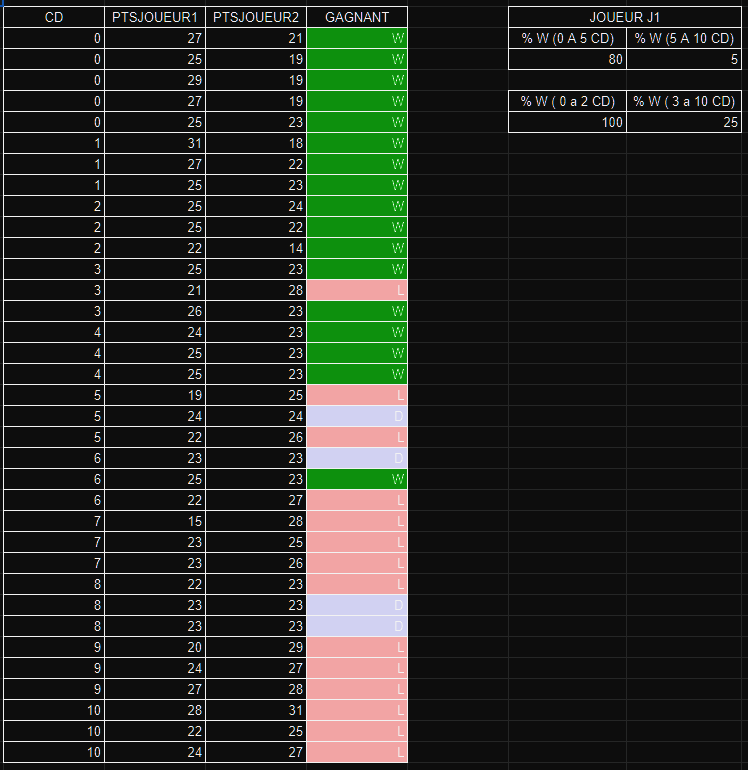
\includegraphics[width=0.70\textwidth]{./TABLEURDEEP1}
\end{center}
\end{figure}
\newpage


\centering \textbf{MinMax 2 vs MinMax 0}
\begin{figure}[!ht]
\begin{center}
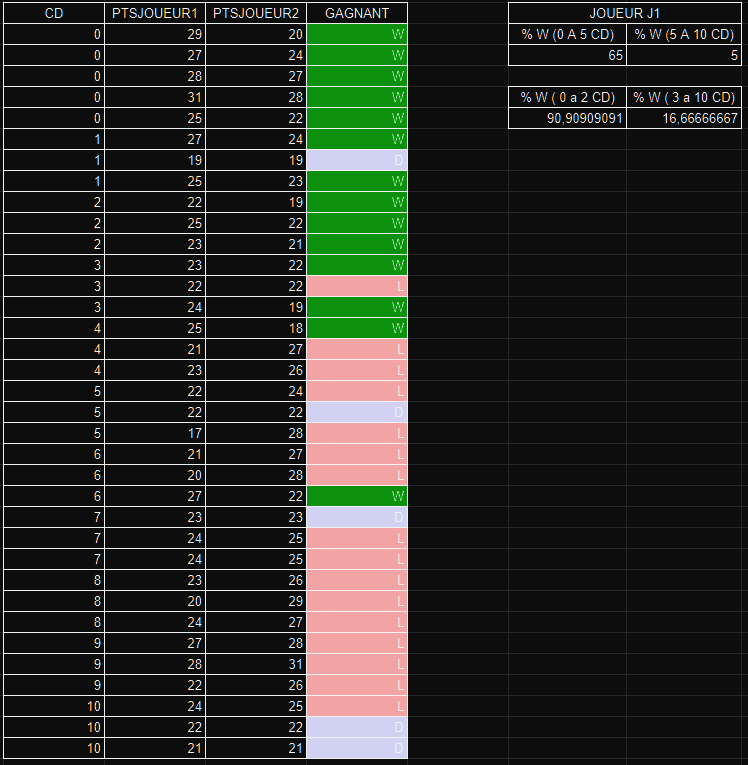
\includegraphics[width=0.70\textwidth]{./TABLEURDEEP2}
\end{center}
\end{figure}
\newpage

\centering \textbf{MinMax 3 vs MinMax 0}
\begin{figure}[!ht]
\begin{center}
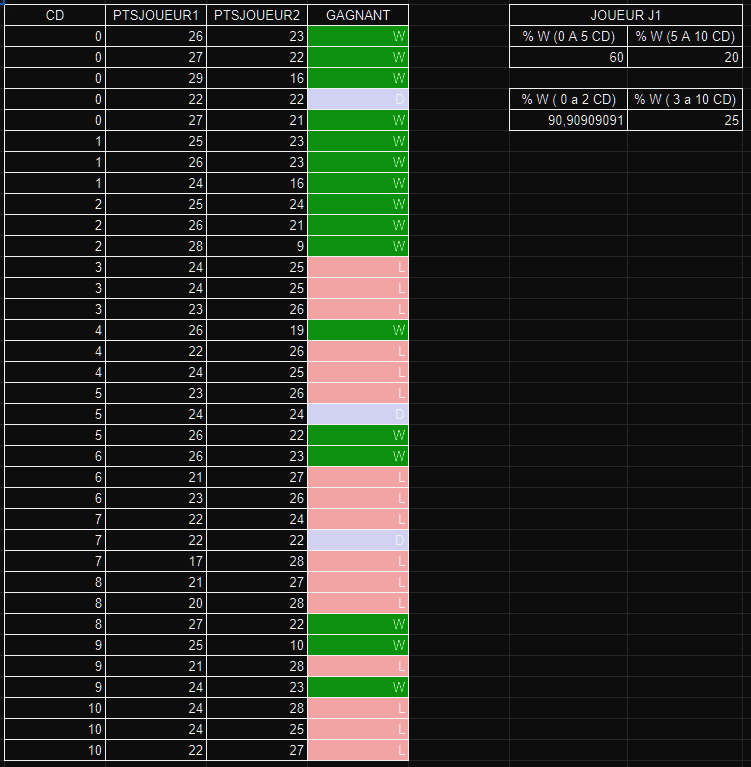
\includegraphics[width=0.70\textwidth]{./TABLEURDEEP3} 
\end{center}
\end{figure}


D'après ces tableaux on peut voir que lorsque l'on donne moins de 3 coups d'avances au joueur MinMax0
MinMax1 gagne toujours. Alors que pour plus de 3 coups d'avances, MinMax0 commencent à battre MinMax1.
Cela fonctionne pareil pour MinMax2 et MinMax3.
Avec des analyses plus poussées, nous aurions pu faire beaucoup d'autre tableur comme ceux-ci, mais 
en changeant la taille de la grille. Grâce a cela nous aurions peu être pu mettre en évidence 
une corrélation entre la taille de la grille et le nombre de coups d'avance.

\newpage
\section{analyse de temps}

Nous avons récupéré des données sur les temps maximums de décisions de MinMax suivant la profondeur
donnée.
Premièrement nous avons afficher a chaque fin de partie le temps maximum de MinMax pour choisir un coup,
le temps total de la partie ainsi que des informations sur le nombre de nœuds parcourus.

\begin{figure}[!ht]
\begin{center}
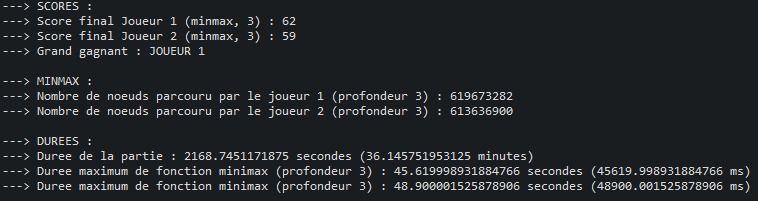
\includegraphics[width=0.70\textwidth]{./EXEMPLEANALYSEFINPARTIE}
\end{center}
\end{figure}

Puis nous avons tracé des courbes après avoir récupéré ces données avec plusieurs profondeurs données :





\begin{figure}[!ht]
\begin{center}
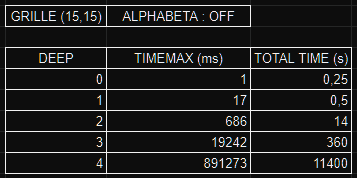
\includegraphics[width=0.70\textwidth]{./TABLEURDONNEESCOURBES} 
\end{center}
\end{figure}

\begin{figure}[!ht]
\begin{center}
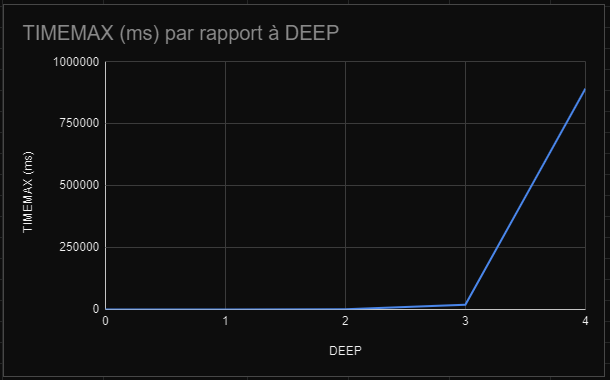
\includegraphics[width=0.70\textwidth]{./TIMEMAXPERDEEP} 
\end{center}
\end{figure}
\newpage

\begin{figure}[!ht]
\begin{center}
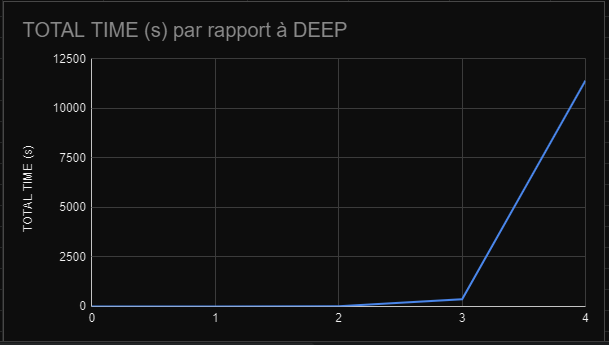
\includegraphics[width=0.70\textwidth]{./TOTALTIMEPERDEEP}
\end{center}
\end{figure}

\textbf{Ces courbes ressemblent fortement aux courbes du 1.1.2, la rapidité du MinMax en temps étant liée au nombre de nœuds parcourus.}





























\chapter{Bilan}

\section{Problèmes rencontrées}

\flushleft La plupart des problèmes étaient liés au MinMax et surtout à la façon de gérer plusieurs objet Board.
En effet, pendant le fonction MinMax, énormément de coups sont joués sur des Boards différentes.
Nous avons donc finit par réussir en comprenant mieux comment fonctionne les objets.
\\
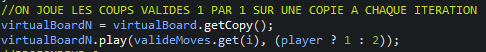
\includegraphics[width=0.60\textwidth]{./VIRTUALBOARD}
\\
Alphabeta ne fut pas implémenté probablement à cause de problème de référencement et de la classe
AlphaBeta. Le problème est peut être aussi le même que lors des premières tentatives d'implémentation
de MinMax. MinMax était incompatible avec notre jeu, il est possible qu'ici AlphaBeta soit incompatible
avec notre version actuelle de MinMax.\\


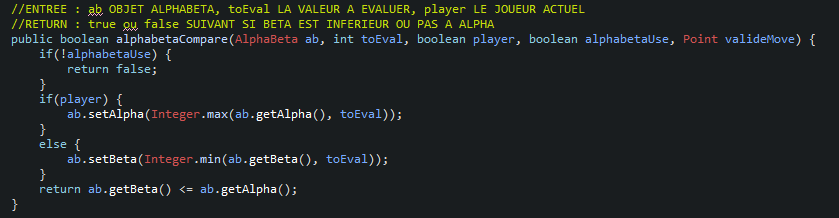
\includegraphics[width=0.60\textwidth]{./ALPHABETA}
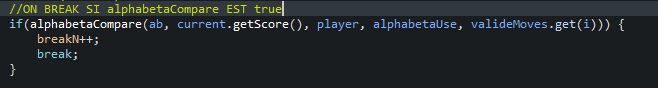
\includegraphics[width=0.60\textwidth]{./ALPHABETA2}

Nous n'avons pas réussit a tracer la courbe nodesperdeep4 car les méthodes pour dessiner la courbe
n'acceptaient pas les BigInteger en paramètre, et le nombre de nœuds total lors d'une partie
jouée par un MinMax4 est supérieur a 2\up{15}. Nous étions donc obligé de récupérer ce nombre dans une
variable BigInteger.
\\
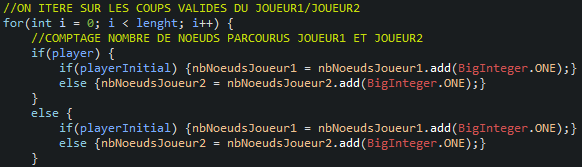
\includegraphics[width=0.60\textwidth]{./BIGINTEGER}
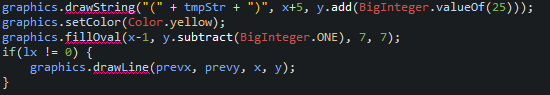
\includegraphics[width=0.60\textwidth]{./BIGINTEGER2}
\\

Le passage de paramètre a Main est différent quand on exécute le programme dans un terminal ou dans
un IDE. Nous avons trouvé comment gérer cela sous Eclipse.
\\
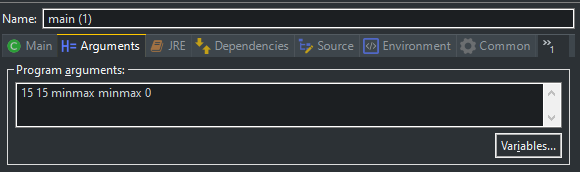
\includegraphics[width=0.60\textwidth]{./MAINPARAM}
\\
\newpage
Enfin, il y avait une redondance du code dans le Main, l'objectif était donc de factoriser le code, pour résoudre ce problème nous avons crée une fonction CurrentPlayer afin de ne pas répéter les opérations du joueur 1 et du joueur 2 

\section{Conclusion}

Ce projet nous a permit de découvrir plusieurs fonctionnalités du langage Java.
Il nous a aussi permit de travailler sur un algorithme très intéressant, et de mieux
comprendre la récursivité ainsi que les structures arborescente.




\newpage


\end{document}